% Web Appendix figure: full decision model input for one unseen-study task (Vaccines), drawn at 16.5 cm.
% Row: covid:vax_choice:p509_p252, as rendered by code/data/base.py:make_view (include_country=False as in the paper's runs). Text is verbatim (no excerpts).
% Build: pdflatex fig_input_vaccines.tex && pdftoppm -png -r 300 -singlefile fig_input_vaccines.pdf fig_input_vaccines
\documentclass[tikz,border=2pt]{standalone}
% Shared look for the pipeline figures. Sizes are final print sizes (no scaling in the manuscript).
% Colors: Okabe-Ito. Blue = model prediction, vermilion = trainable theta, dark gray = human / data.
\usepackage[T1]{fontenc}
\usepackage{lmodern}
\usepackage{amsmath,amssymb,bm}
\usepackage{array}
\renewcommand{\familydefault}{\sfdefault}
\usetikzlibrary{positioning,arrows.meta,calc,fit,backgrounds}
\pgfdeclarelayer{back}\pgfsetlayers{back,background,main}

\definecolor{cpred}{HTML}{0072B2}
\definecolor{ctrain}{HTML}{D55E00}
\definecolor{chuman}{HTML}{333333}
\definecolor{cline}{HTML}{555555}
\definecolor{cfield}{HTML}{F2F2F2}
\definecolor{cframe}{HTML}{BBBBBB}
\definecolor{ctok}{HTML}{007A5A}  % Okabe-Ito bluish green, darkened: special tokens

\tikzset{
  >={Stealth[length=3.5pt]},
  every node/.append style={execute at begin node={\hyphenpenalty=10000\exhyphenpenalty=10000}},
  flow/.style={->, line width=0.6pt, draw=cline},
  pred/.style={->, line width=0.9pt, draw=cpred},
  grad/.style={->, line width=0.8pt, draw=ctrain, dash pattern=on 3pt off 2pt},
  panel/.style={draw=cframe, line width=0.5pt, rounded corners=3pt},
  ptitle/.style={font=\footnotesize\bfseries, anchor=north west, inner sep=0pt},
  raw/.style={draw=cframe, fill=white, rounded corners=1.5pt, font=\scriptsize, align=left, inner sep=2.5pt},
  field/.style={draw=cline, fill=cfield, rounded corners=1.5pt, font=\scriptsize, align=left, inner sep=2.5pt},
  box/.style={draw=cline, fill=white, rounded corners=2pt, align=center, font=\footnotesize, inner sep=2.5pt},
  predbox/.style={box, draw=cpred, line width=0.8pt},
  humanbox/.style={box, draw=chuman, line width=0.8pt},
  trainbox/.style={box, draw=ctrain, line width=0.9pt},
  rawtxt/.style={raw, draw=none, fill=none},
  fieldtxt/.style={field, draw=none, fill=none},
  note/.style={font=\scriptsize, text=black!70, align=left, inner sep=0pt, anchor=north west},
}
\newcommand{\tok}[1]{\textcolor{ctok}{\textbf{\texttt{#1}}}}
% \rowboxes{raw node}{field node}{bottom coordinate}: draws both boxes down to the lower of the two bottoms,
% so a raw item and its input field always have the same height, and links them with an arrow at mid-height.
\newcommand{\rowboxes}[3]{%
  \path let \p1=(#1.south), \p2=(#2.south), \n1={min(\y1,\y2)} in coordinate (#3) at (0,\n1);
  \begin{scope}[on background layer]
    \draw[raw]   (#1.north west) rectangle (#1.east |- #3);
    \draw[field] (#2.north west) rectangle (#2.east |- #3);
  \end{scope}
  \coordinate (#3-mid) at ($(#1.north east)!0.5!(#1.east |- #3)$);
  \draw[flow] (#3-mid) -- (#3-mid -| #2.west);
}


\begin{document}
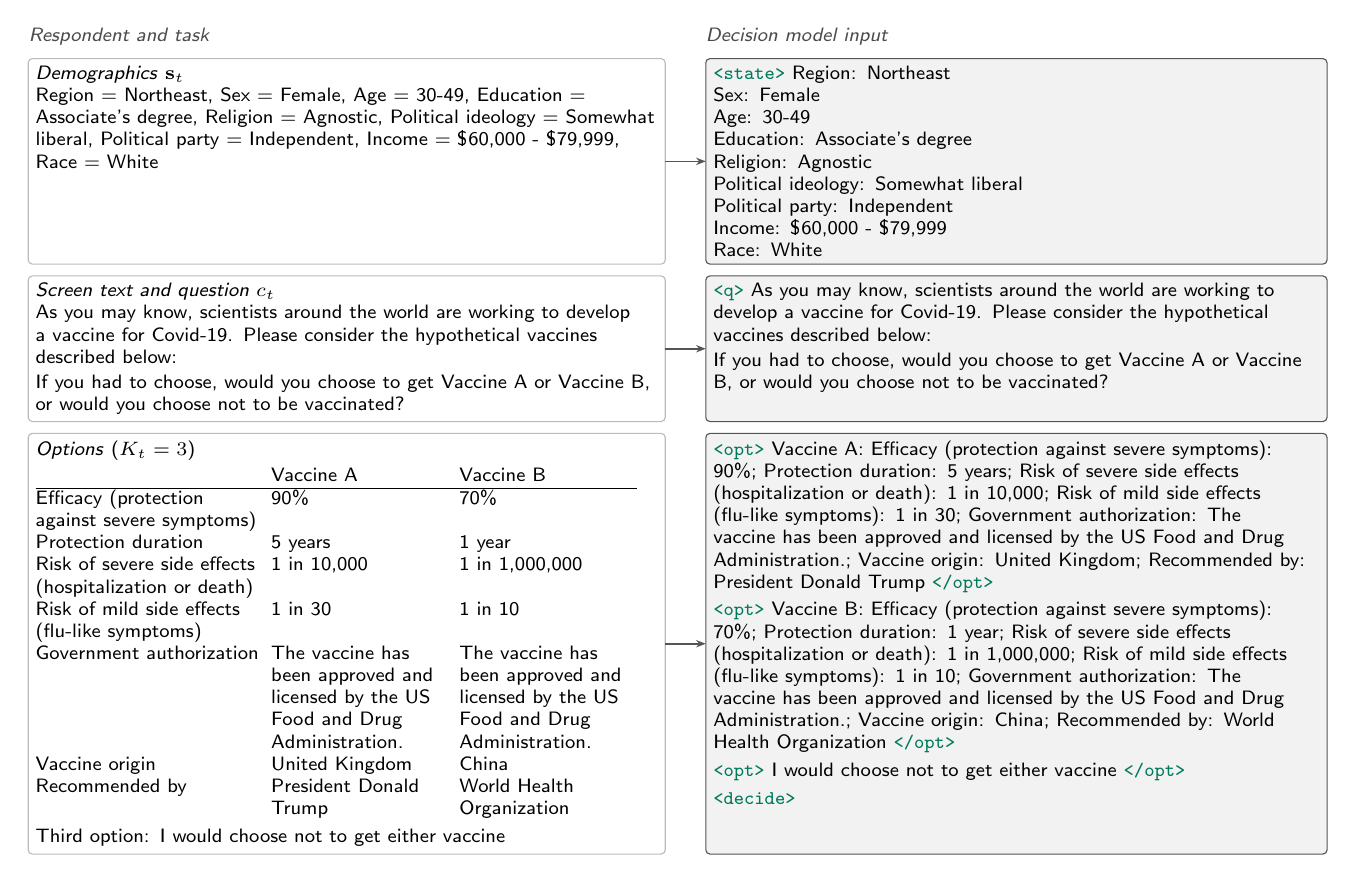
\begin{tikzpicture}

\node[note, font=\scriptsize\itshape] at (0,0) {Respondent and task};
\node[note, font=\scriptsize\itshape] at (8.6,0) {Decision model input};

\coordinate (inx) at (12.55,0);
\node[rawtxt, text width=7.9cm, anchor=north west] (rs) at (0,-0.4) {%
  \textit{Demographics} $\mathbf{s}_t$\\
  Region = Northeast, Sex = Female, Age = 30-49, Education = Associate's degree,
  Religion = Agnostic, Political ideology = Somewhat liberal, Political party = Independent,
  Income = \$60,000 - \$79,999, Race = White};
\node[fieldtxt, text width=7.7cm, anchor=north] (fs) at (rs.north -| inx) {%
  \tok{<state>} Region: Northeast\\ Sex: Female\\ Age: 30-49\\ Education: Associate's degree\\
  Religion: Agnostic\\ Political ideology: Somewhat liberal\\ Political party: Independent\\
  Income: \$60,000 - \$79,999\\ Race: White};
\rowboxes{rs}{fs}{b1}
\node[rawtxt, text width=7.9cm, anchor=north west] (ri) at ($(b1)+(0,-0.15)$) {%
  \textit{Screen text and question} $c_t$\\
  As you may know, scientists around the world are working to develop a vaccine for Covid-19.
  Please consider the hypothetical vaccines described below:\\[1pt]
  If you had to choose, would you choose to get Vaccine A or Vaccine B, or would you choose not to be vaccinated?};
\node[fieldtxt, text width=7.7cm, anchor=north] (fi) at (ri.north -| inx) {%
  \tok{<q>} As you may know, scientists around the world are working to develop a vaccine for Covid-19.
  Please consider the hypothetical vaccines described below:\\[1pt]
  If you had to choose, would you choose to get Vaccine A or Vaccine B, or would you choose not to be vaccinated?};
\rowboxes{ri}{fi}{b2}
\node[rawtxt, text width=7.9cm, anchor=north west] (rc) at ($(b2)+(0,-0.15)$) {%
  \textit{Options} ($K_t = 3$)\\[1pt]
  \begin{tabular}{@{}>{\raggedright\arraybackslash}p{2.85cm}@{\hspace{4pt}}>{\raggedright\arraybackslash}p{2.25cm}@{\hspace{4pt}}>{\raggedright\arraybackslash}p{2.25cm}@{}}
                                                     & Vaccine A & Vaccine B \\ \hline
  Efficacy (protection against severe symptoms)      & 90\%      & 70\% \\
  Protection duration                                & 5 years   & 1 year \\
  Risk of severe side effects (hospitalization or death) & 1 in 10,000 & 1 in 1,000,000 \\
  Risk of mild side effects (flu-like symptoms)      & 1 in 30   & 1 in 10 \\
  Government authorization                           & The vaccine has been approved and licensed by the US Food and Drug Administration. & The vaccine has been approved and licensed by the US Food and Drug Administration. \\
  Vaccine origin                                     & United Kingdom & China \\
  Recommended by                                     & President Donald Trump & World Health Organization \\
  \end{tabular}\\[2pt]
  Third option: I would choose not to get either vaccine};

\node[fieldtxt, text width=7.7cm, anchor=north] (fc) at (rc.north -| inx) {%
  \tok{<opt>} Vaccine A: Efficacy (protection against severe symptoms): 90\%; Protection duration: 5 years;
  Risk of severe side effects (hospitalization or death): 1 in 10,000; Risk of mild side effects (flu-like symptoms): 1 in 30;
  Government authorization: The vaccine has been approved and licensed by the US Food and Drug Administration.;
  Vaccine origin: United Kingdom; Recommended by: President Donald Trump \tok{</opt>}\\[2pt]
  \tok{<opt>} Vaccine B: Efficacy (protection against severe symptoms): 70\%; Protection duration: 1 year;
  Risk of severe side effects (hospitalization or death): 1 in 1,000,000; Risk of mild side effects (flu-like symptoms): 1 in 10;
  Government authorization: The vaccine has been approved and licensed by the US Food and Drug Administration.;
  Vaccine origin: China; Recommended by: World Health Organization \tok{</opt>}\\[2pt]
  \tok{<opt>} I would choose not to get either vaccine \tok{</opt>}\\[2pt]
  \tok{<decide>}};
\rowboxes{rc}{fc}{b3}


\end{tikzpicture}
\end{document}
